% Copyright (C)  2016  Orestis Malaspinas.
%     Permission is granted to copy, distribute and/or modify this document
%     under the terms of the GNU Free Documentation License, Version 1.3
%     or any later version published by the Free Software Foundation;
%     with no Invariant Sections, no Front-Cover Texts, and no Back-Cover Texts.
%     A copy of the license can be downloaded from:
%     https://www.gnu.org/licenses/fdl.html.

\documentclass[a4paper,12pt]{book}
\usepackage[utf8]{inputenc}
\usepackage[french]{babel}
\usepackage{amsfonts,bm,amsmath,amssymb,graphicx,amsthm}
\usepackage{cancel}
\usepackage{mathtools}
\usepackage{caption}
\usepackage{hyperref}

\setlength{\parindent}{0pt}

\newcommand{\real}{\mathbb{R}}
\newcommand{\integer}{\mathbb{Z}}
\renewcommand{\natural}{\mathbb{N}}
\newcommand{\complex}{\mathbb{C}}
\newcommand{\zbar}{\bar{z}}
\newcommand{\dd}{\mathrm{d}}
\newcommand{\perm}{\mathrm{perm}}
\newcommand{\card}{\mathrm{card}}
\newcommand{\fh}{\hat{f}}
\newcommand{\gh}{\hat{g}}
\newcommand{\hh}{\hat{h}}
\renewcommand{\Re}{\mathrm{Re}}
\renewcommand{\Im}{\mathrm{Im}}
\newcommand{\pDeriv}[2]{\frac{\partial #1}{\partial #2}}
\newcommand{\pDerivTwo}[2]{\frac{\partial^2 #1}{\partial #2^2}}
\newcommand{\dDeriv}[2]{\frac{\dd #1}{\dd #2}}
\newcommand{\dDerivTwo}[2]{\frac{\dd^2 #1}{\dd #2^2}}
\newtheorem{definition}{Définition}
\newtheorem*{exemples}{Exemples}
\newtheorem*{exemple}{Exemple}
\newtheorem*{solution}{Solution}
\newtheorem{exercice}{Exercice}
\newtheorem*{remarque}{Remarque}
\newtheorem{proprietes}{Propriétés}
\newtheorem{theoreme}{Théorème}
\newcommand{\cm}{\mathrm{cm}}
\newcommand{\km}{\mathrm{km}}
\newcommand{\mm}{\mathrm{mm}}
\newcommand{\cd}{\mathrm{cd}}
\newcommand{\mol}{\mathrm{mol}}
\newcommand{\m}{\mathrm{m}}
\newcommand{\s}{\mathrm{s}}
\newcommand{\kg}{\mathrm{kg}}
\newcommand{\g}{\mathrm{g}}
\newcommand{\K}{\mathrm{K}}
\newcommand{\J}{\mathrm{J}}
\newcommand{\C}{\mathrm{C}}
\newcommand{\A}{\mathrm{A}}
\newcommand{\N}{\mathrm{N}}
\newcommand{\atm}{\mathrm{atm}}
\renewcommand{\bar}{\mathrm{bar}}
\newcommand{\V}{\mathrm{V}}
\newcommand{\W}{\mathrm{W}}
\newcommand{\Pa}{\mathrm{Pa}}


\title{Résumé du cours de Physique Générale}
\author{Orestis Malaspinas}

\begin{document}
\maketitle

\chapter*{Avertissement}

Cette tentative de polycopié contient certainement un grand nombre d'erreurs étant donné qu'elle est développée 
en même temps que le cours est donné et qu'elle en est à ses premiers mois de vie. 
Quand vous trouverez des erreurs n'hésitez pas à me les communiquer
et ainsi améliorer la qualité de ce polycopié. Toute erreur trouvée concernant de la ``physique'' (pas les fautes
d'orthographe donc) seront récompensées par un bonus sur la note des contrôles continus.

\chapter*{Bibliographie}

Il existe une multitude de bons livres de physique générale à disposition. Ce polycopié est largement inspiré du livre 
de D. C. Giancoli, \textit{Physics: principles with applications},
7-th edition, Pearson, 2014. D'autres lectures possibles sont les suivantes:
\begin{itemize}
	\item Walker, Halliday \& Resnick, Fundamentals of Physics, Wiley, 2014.
	\item E. Hecht, Physique, 1999.
\end{itemize}
Une partie de la bibliographie que je vous ai donné est en anglais. 
Il existe des traductions qui sont en principe disponibles à 
la bibliothèque. 

\chapter{Mesures, incertitudes, et estimations}

Pour celles et ceux qui sont intéressés par plus de détails, vous pouvez vous référer au cours de métrologie de l'EPFL par exemple: \url{http://sb.epfl.ch/page-52191-en.html}

\section{Généralités}

Toues les sciences ``naturelles'' sont basées sur \textit{l'observation} du monde qui nous entoure. 
Mais malgré le fait qu'on ait l'impression que le processus d’observation soit une suite simple:
observation, expérimentation, obtention de résultats, qu'on explique avec une \textit{théorie} (un ensemble de \textit{lois}) cela n'est pas vraiment le cas. En fait,
de façon proche à ce qui se passe dans les arts, les sciences sont un processus hautement créatif. 
En effet, lors d'une observation un scientifique ne décrit pas tout ce qu'il voit, 
mais sélectionne uniquement ce qu'il juge important
pour la compréhension et l'interprétation d'un phénomène. De plus, une fois sélectionné
le processus à observer, il convient de créer une expérience permettant de le mesurer de façon aussi précise que possible
pour pouvoir le décrire. La mesure tient donc une place centrale dans les sciences et se complète parfaitement avec la création de théories
qui permettent l'explication d'observations. Par ailleurs, toutes les théories ne sont pas le fruit
d'expériences (ou d'observations) mais ont souvent été le résultat de constructions de l'esprit. 
Dans ce cas les expériences, viennent confirmer (ou infirmer) les théories. En effet, une théorie physique est
supposée vraie jusqu'à ce qu'une expérience vienne l'infirmer (on ne peut pas prouver une théorie).

Les expériences ont donc deux fonctions principales
\begin{itemize}
 \item Collecter des données qui permettront la dérivation de lois physiques.
 \item Vérifier ou infirmer les lois physiques.
\end{itemize}

Les lois physiques sont des outils très pratiques permettant la prédiction \textit{quantitative} 
de phénomènes (et non la ``post-diction'' comme avec les expériences). Il est par exemple possible de prédire très précisément la hauteur à laquelle il faut lancer un satellite 
pour qu'il se retrouve en orbite géostationnaire (et donc connaître la quantité de carburant nécessaire par exemple) grâce aux lois de Newton. 
Ce qui serait certainement beaucoup plus difficile à déterminer expérimentalement, s'il fallait faire des dizaines d'essais jusqu'à ce que ça marche.

Par ailleurs, beaucoup de ``lois'' ont des capacités prédictives mais ne sont pas complètement générales. Par exemple, bien que les lois de Newton 
marchent très très bien pour notre vie de tous les jours, certaines applications d'usage quotidien ne fonctionneraient pas si on s'en tenait là. 
En effet, le GPS requiert l'extension des lois de Newton à la relativité générale pour pouvoir fonctionner correctement. En fait
la gravitation Newtonienne est une approximation de la relativité générale.

Ces approximations sont souvent le résultat de simplifications faites dans la représentation dont ont se fait 
de processus physiques: les \textit{modèles}. Un modèle est une vision de l'esprit qui permet de réunir plusieurs
situations qui à première vue peuvent paraître non-semblables ou à simplifier un problème afin de pouvoir le résoudre plus simplement. 
Par exemple un liquide est composé d'atomes qui se déplacent. Il serait possible (mais complètement infaisable et inutile dans presque tous les cas) 
d'étudier chaque atome individuellement pour avoir une description très détaillée du mouvement d'un fluide. Néanmoins, il est beaucoup plus simple de 
faire \textit{l'hypothèse} qu'un fluide peut être considéré comme un objet continu.

\section{Mesure et incertitude}

Comme nous venons de le dire les mesures tiennent une place primordiale en physique. Mais toute mesure ne peut être 
parfaite et contient donc une part d'incertitude. En générale l'incertitude d'une mesure provient 
de la précision limitée des instruments utilisés. Par exemple, lors de la mesure d'une longueur avec une règle,
la graduation est en générale faite à chaque millimètre. Il est donc impossible d'être plus précis
que le millimètre (on pourrait éventuellement dire qu'on est précis à 0.5 millimètres, mais il faudrait pour cela que l'utilisateur de la 
règle ait de très très très bons yeux, que le fabriquant de la règle ait un processus absolument parfait de graduation, etc).
Si la longueur, $L$, d'un objet mesuré à la règle est de $10.1\cm$, on peut donner l'information de l'incertitude 
en ajoutant derrière le sigle $\pm 0.1\cm$ ou
\begin{equation*}
 L=10.1\pm0.1\ \cm.
\end{equation*}
Cela signifie que la valeur de $L$ est située quelque part entre $10$ et $10.2$ centimètres.
Une autre façon de mesurer la précision d'une mesure est de donner l'erreur en pourcentage de la mesure effectuée.
Ici nous aurions que l'erreur est de
\begin{equation*}
 \frac{0.1}{10.1}\cdot 100\cong 1\%.
\end{equation*}
Cette façon de quantifier l'erreur dépend donc de la valeur de la quantité mesurée (plus la longueur mesurée est grande plus
le pourcentage sera petit et inversement).


Une autre source d'incertitude peut provenir de la nature du phénomène observé. Si nous mesurions aujourd'hui la température 
à un endroit donné de Genève durant toute la journée nous verrions une certaine courbe de température. Cette courbe serait certainement
différente de la courbe du lendemain ou de celle du même jour de l'année d'après. Ces mesures non reproductibles 
doivent donc faire l'objet d'études statistiques et contiennent des incertitudes de nature très différentes (en plus des erreurs dues aux mesures
elles-mêmes).

\subsection{Chiffres significatifs}

Le nombre de chiffres significatifs est le nombre de chiffres d'un résultat dont la valeur est ``sûre''. Le nombre $1.23$ contient trois chiffres 
significatifs tout comme le nombre $0.0123$ (les zéros ne sont là que pour placer la virgule). La façon dont on donne un résultat
permet donc d'indiquer avec quelle précision nous connaissons un résultat. Il est souvent tentant d'exprimer un résultat avec un grand nombre de chiffres
significatifs, mais cela peut s'avérer extrêmement contre productif car cela donne une fausse impression de grande précision d'une mesure.
Si nous reprenons notre mesure avec la règle de la longueur $L=10.1$. En se donnant un peu de peine on peut facilement se convaincre qu'on a
pas exactement $10.1$ mais un peu plus disons $10.15$. Même si cela n'est pas vraiment grave dans ce cas, le $5$ est totalement superflu
car il est complètement impossible de dire si cela est 10.15 ou 10.13 ``à l’œil''. De façon générale si notre précision avait été de $\pm 1\cm$
on aurait écrit $L=10$, à $\pm 0.1$ on écrit $10.1$, à $\pm 0.01$ on écrit $10.10$, etc. Par ailleurs, lorsqu’on combine des valeurs contenant
des incertitudes il faut également faire attention. Supposons que nous ayons un carré dont le coté fait $10.1\cm$, sa surface est de 
$10.1^2=102.01$. Hors, la valeur de la surface est incluse entre les deux valeurs extrêmes possibles: $10^2=100$ et $10.2^2=104.04$. Il est 
donc inutile de garder $0.01$ et on donne la valeur de $102$ pour la surface.

Il est commun d'écrire les nombre en \textit{notation scientifique} ou en puissances de $10$. Le nombre $10'100$ s'écrit $1.01\cdot 10^4$ en notation
scientifique, le nombre $0.001234=1.234\cdot 10^{-3}$, ... Un des avantages de la notation scientifique, c'est qu'elle permet immédiatement de connaître le nombre de chiffres
significatifs d'un résultat: il correspond au nombre de chiffres composant le nombre multiplié par la puissance de $10$.

\section{Unités, Système International}

Toute mesure doit être effectuée par rapport à un ``standard'' ou unités. Cela n'a aucun sens de dire qu'un éléphant pèse 36, si nous ne disons pas
36 en quelles unités. Pour chaque grandeur de multiple standards ont été créé au cours des années qui sont devenus de plus en plus précis
avec les avancées technologiques (combien exactement mesure $1\m$, la durée d'une seconde, etc). 
Dans cette section nous allons discuter les unités des grandeurs de base  de la physique. Nous verrons en particulier le \textit{Système International} (ou SI).

Ne pas se mettre d'accord sur un système d'unités peut avoir des conséquences catastrophiques. Un exemple récent 
est la perte du satellite Mars Climate Orbiter (le coût de la mission était de 330 millions de dollars) 
qui a explosé alors qu'il essayait de se mettre en orbite autour de Mars,
car une partie du code informatique récoltant les donnée de la sonde donnait des résultats en unités 
non-SI alors que la NASA travaillait en SI. Il y a donc eu une très grossière erreur dans le calcul
de la trajectoire à adopter pour la mise en orbite et le satellite s'est écrasé (plus de détails ici par exemple \url{https://fr.wikipedia.org/wiki/Mars_Climate_Orbiter}).

Les unités sont définies par rapport à des grandeurs ``facilement'' mesurables avec une grade précision et qui ne changent pas (ou très très très peu)
au cours du temps.

\subsection{Longueur}

Le standard international fût établi par la France dans les années 1790. 
Pour les unités de longueur est le mètre (abrégé $\m$). A l'origine le mètre était 1/10'000'000 de la distance entre l'équateur et un des pôles.
A partir de cette mesure un étalon en platine fût forgé (c'est quand même plus pratique à utiliser). Puis, en 1889, le mètre a été défini comme la distance entre deux très fines encoche sur une barre d'un alliage platine-iridium. Comme cette façon de définir le mètre n'était pas suffisamment précise pour beaucoup d'applications, en 1960
le mètre devint $1'650'763.73$ longueur d'onde d'une lumière émise par le gaz krypton-86. En 1983, fût redéfini comme la distance parcourue par la lumière en 1/299'792'458 secondes.

Il existe d'autres unités de longueur, par exemple les britanniques utilisent le pouce  ou inch (1$\mathrm{in.}$ correspond à 0.0254$\m$). Dans ce cours nous nous concentrerons principalement
sur le système SI.

\subsection{Temps}

La mesure du temps en SI est donnée en secondes (abrégée $\s$). Une seconde a longtemps été définie comme étant $1/(3600\cdot 24)=1/86'000$-ème
de journée solaire. La vitesse de rotation de la terre se ralentissant légèrement d'année en année, il a été nécessaire de raffiner de plus en plus 
cette définition. A présent une seconde correspond à un processus atomique. Il s'agit du temps nécessaire à 9'192'631'770 de 
la transitions entre deux états de l'atome de césium 133. 

\subsection{Masse}

Le kilogramme (abrégé $\kg$) est la masse d'un étalon international du kilogramme. En 1795, le kilogramme était la d'un décimètre cube 
d'eau à une température de $4^\circ\C$. Puis il a été remplacé par un étalon en platine iridié (voir Fig.~\ref{fig_kg}). Il s'agit de la seule unité utilisant encore un étalon, 
aucune ``grandeur naturelle'' n'ayant pu être utilisée pour définir le kilogramme autrement. Des copies de cet étalon ont été fabriquée et envoyées à
chaque état qui en ont fait d'autres copies officielles pour contrôler les balances utilisées un peu partout sur les territoires.
\begin{figure}
\begin{center}
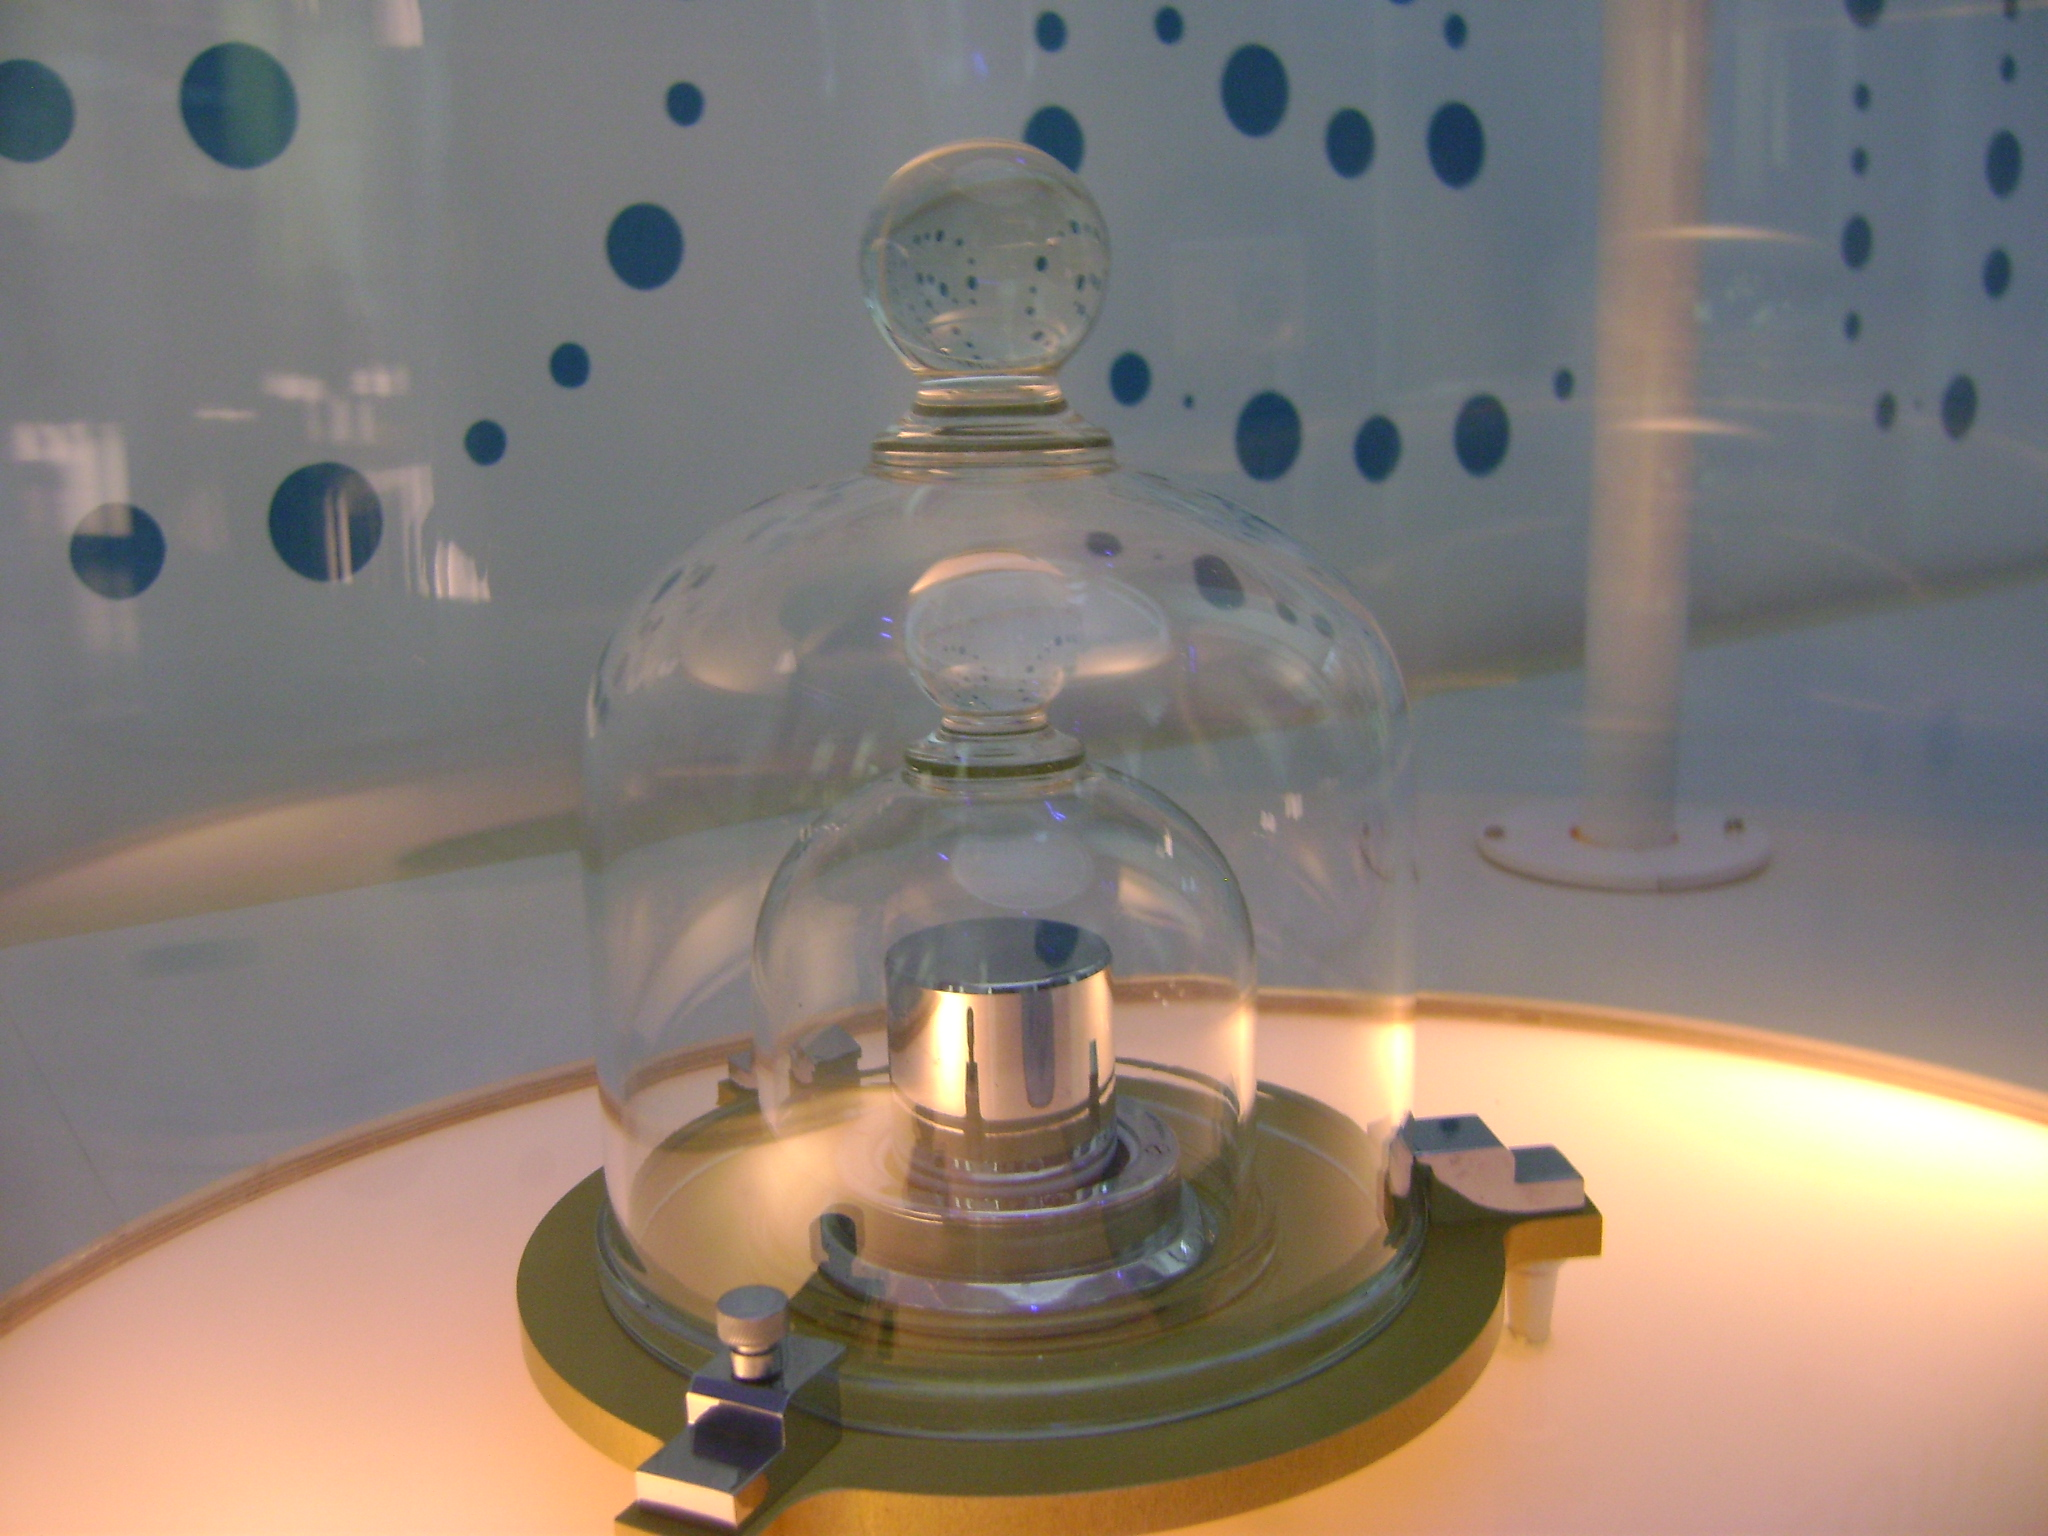
\includegraphics[width=0.5\textwidth]{figs/kilogram_replica.jpg}
\caption{Une réplique de l'étalon international du kilogramme présentée à la cité des sciences et de l'industrie (Vilette), source: \url{https://upload.wikimedia.org/wikipedia/commons/a/ac/Prototype_kilogram_replica.JPG}}
\label{fig_kg}
\end{center}
\end{figure}

\subsection{Température}

La température mesure le degré d'échauffement d'un corps. En SI l'unité de la température est le degré Kelvin (abrégé $\K$).
Il est défini comme le $1/273.16$-ème de la température du point triple de l'eau (la température où les trois phases, solides, liquides, gazeuse, de l'eau 
peuvent coexister en équilibre thermodynamique). Cette température se trouve par définition à $273.16^\circ\K$ ou encore à $0.01^\circ\C$.
Nous verrons un peu plus de détails sur la définition du zéro degrés Kelvin (ou zéro absolu) dans la suite du cours.

\subsection{Courant}

L'intensité du courant électrique est mesurée en Ampères (abrégé $\A$). Un ampère est l'intensité de courant constant qui circulerait 
dans deux fils conducteurs infinis placés dans le vide, de section négligeable, et placés à une distance d'un mètre l'un de l'autre 
qui produirait une force de $2\cdot 10^{-7}$ Newton par longueur de mètre. Les autres unités très utiles en électricité, l'ohm (abrégé $\Omega$) et 
le volt (abrégé $\V$) se déduisent ensuite par les fameuse formules $U=R\cdot I$ ($[\V]=[\Omega]\cdot [\A]$) et $P=U\cdot I$ ($[\W]=[\V]\cdot [\A]$).

\subsection{Quantité de matière}

La quantité de matière se mesure en moles (abrégé $\mol$). Une mole de matière contient autant de particules que 
$0.012\kg$ contient d'atomes de Carbone 12 soit environ $6.02\cdot 10^{23}$ atomes (on appelle ce nombre, le nombre d'Avogadro ou de Loschmidt). 
Cette valeur est étonnamment constante. Pour
tout élément du tableau périodique une mole sera le nombre d'atomes d'élément de poids atomique $N$ (ou $N$ unités de masse atomique), dans $N$ grammes de matière.

\subsection{Intensité lumineuse}

L'intensité lumineuse est mesurée en candela (abrégé $\cd$). Elle est donnée par l'intensité lumineuse émise par
une source monochromatique de fréquence de $540\cdot 10^{12}\s^{-1}$ et dont l'intensité énergétique est de 
$1/683 \W$ par stéradian (équivalent du radian mais sur une sphère). L'intensité lumineuse représente la puissance (la quantité d'énergie 
par unité de temps) émise par une source par angle solide. 

A titre de comparaison, un candela est environ l'intensité 
lumineuse émise par une bougie normale. Ou encore, une ampoule led typique 
à faible consommation électrique (15 Watts) produit environ 10$\cd$.

\subsection{Préfixes du Système International}

Pour exprimer les puissances de 10 du SI, un certain nombre de préfixes ont été définis pour simplifier 
les notations (voir la Table~\ref{table_prefixe}). Il est relativement aisé de convertir entre les différents préfixes.
Ainsi $23\cm$ correspondent à $230\mm$ ou $0.23\m$. Pour le calcul de surfaces (ou d'unités prises à une certaine puissance les choses
se compliquent un tout petit peu. Ainsi le préfixe est complètement attaché à l'unité. Par exemple les unités d'un volume
se convertissent comme
\begin{equation}
 23\cm^3=23\cdot(10^{-2} m)^3=23\cdot 10^{-6}m^3.
\end{equation}

\begin{table}
\begin{tabular}{|l|l|l|l|l|}
\hline
$10^n$&Préfixe français&Symbole&Nombre décimal&Désignation\\
\hline\hline
$10^{24}$&yotta&Y&1 000 000 000 000 000 000 000 000&Quadrillion\\
\hline
$10^{21}$&zetta&Z&1 000 000 000 000 000 000 000&Trilliard\\
\hline
$10^{18}$&exa&E&1 000 000 000 000 000 000&Trillion\\
\hline
$10^{15}$&péta&P&1 000 000 000 000 000&Billiard\\
\hline
$10^{12}$&téra&T&1 000 000 000 000&Billion\\
\hline
$10^{9}$&giga&G&1 000 000 000&Milliard\\
\hline
$10^{6}$&méga&M&1 000 000&Million\\
\hline
$10^{3}$&kilo&k&1 000&Millier\\
\hline
$10^{2}$&hecto&h&100&Centaine\\
\hline
$10^{1}$&déca&da&10&Dizaine\\
\hline
$10^{0}$&(aucun)&—&1&Unité\\
\hline
$10^{-1}$&déci&d&0,1&Dixième\\
\hline
$10^{-2}$&centi&c&0,01&Centième\\
\hline
$10^{-3}$&milli&m&0,001&Millième\\
\hline
$10^{-6}$&micro&$\mu$&0,000 001&Millionième\\
\hline
$10^{-9}$&nano&n&0,000 000 001&Milliardième\\
\hline
$10^{-12}$&pico&p&0,000 000 000 001&Billionième\\
\hline
$10^{-15}$&femto&f&0,000 000 000 000 001&Billiardième\\
\hline
$10^{-18}$&atto&a&0,000 000 000 000 000 001&Trillionième\\
\hline
$10^{-21}$&zepto&z&0,000 000 000 000 000 000 001&Trilliardième\\
\hline
$10^{-24}$&yocto&y&0,000 000 000 000 000 000 000 001&Quadrillionième\\
\hline
\end{tabular}
\caption{Préfixes du Système international d'unités et noms des nombres correspondants.}
\label{table_prefixe}
\end{table}

\begin{exercice}{Conversion d'unités}

\begin{enumerate}
\item Écrivez en mètres les grandeurs suivantes: $1\cm$, $1.23\cdot 10^6\mu\m$, $72\mathrm{da}\m$.
\item Ajoutez les grandeurs suivantes $3\mu\g$, $7\mathrm{d}\g$, $120\kg$. Écrivez les en notation scientifique avec 
trois chiffres significatifs.
\item Calculez le produit des grandeurs suivantes $8.76\m$, $5.43\mm$, $2.10\mu\m$. Que représente ce produit?
Écrivez le résultat en $\m^3$ et en $\cm^3$.
\item Le rayon d'un atome d'oxygène est d'environ $60\mathrm{pm}$. Combien d'atomes posés côte à côte faudrait-il
pour faire $1\m$? A combien de $\mol$ cela correspondrait-il?
\item Classez ces grandeurs par ordre croissant $1\mm$, $1\cm$, $1\m$, $1\mathrm{dam}$, $1\mathrm{pm}$, et $1\mathrm{dm}$.
\end{enumerate}
\end{exercice}

\begin{exercice}{Préfixes SI}

\begin{enumerate}
\item Exprimez en utilisant les préfixes SI et le moins de chiffre possible les nombres suivants
\begin{equation*}
3\cdot 10^6\kg,\quad 4\cdot10^{-9}\m,\quad 56\cdot10^{-13}\s,\quad 78\cdot 10^{14} \mathrm{A},\quad 0.56\cdot 10^1 \mathrm{K} ,\quad 912\cdot10^{19}\mol.
\end{equation*}
\item On estime que le cerveau humain peut stocker environ cent mille milliards de bits d’informations.
\begin{enumerate}
	\item Écrire ce nombre en forme décimale.
	\item En notation scientifique.
	\item Exprimer ce nombre en ajoutant un préfixe au mot bit.
	\item Sachant qu'un byte correspond à 8bits, combien de bytes cela fait-il?
\end{enumerate}
\end{enumerate}
\end{exercice}


\section{Ordre de grandeur}

Souvent nous pouvons vouloir qu'une estimation rapide d'une quantité ou simplement vouloir rapidement avoir une idée 
de comment ``marche'' un processus. Pour ce faire plutôt que d'entrer complètement dans tous les détails compliqués des calculs
il peut être beaucoup plus simple de fonctionner avec des ordres de grandeurs de nos quantité (en gros on arrondit tout à l'entier ou même 
à la puissance de 10)\footnote{Cela peut être très pratique quand on fait ses courses pour savoir s'il y a une erreur grossière sur le montant qu'on paie.}.
On a donc un résultat précis ``à la puissance de 10 près''. 
\begin{exercice}{Volume d'un lac}

 Calculez le volume du lac Léman sachant qu'il fait environ $70\km$ de long pour $10\km$ de large et $100\m$ de profondeur.\footnote{Selon le site: \url{http://ge.ch/eau/lac-leman} le volume véritable du lac est de $89$ milliards de mètres cubes. Sa longueur est de $73\km$, sa largeur est de $14\km$ et sa profondeur moyenne est de $150.4\m$.}
\end{exercice}
\begin{exercice}{Hauteur d'un bâtiment}

Je souhaite estimer la hauteur d'un bâtiment. Supposons que mes yeux soient à une hauteur de $1.5\m$ du sol. La seule information connue est que quand je me place 
à une distance d'un écartement de bras d'un arbre (mesurant environ $3\m$ de haut et se trouvant à $20$ pas du bâtiment) placé entre moi et le bâtiment, 
l'arbre cache tout juste le haut du bâtiment.
\end{exercice}

\begin{exercice}{Épaisseur d'une feuille de papier}

Vous avez à disposition une règle (précise au millimètre) et un livre. 
Estimez aussi précisément que possible et avec un minimum d'effort
l'épaisseur d'une feuille du livre.
\end{exercice}

\section{Analyse dimensionnelle}

Lorsque nous parlons de dimensions d'une quantité, nous nous référons souvent au type des unités de la quantité. Une longueur 
sera représentée par $[L]$\footnote{Une lettre représentant la quantité entourée de crochets.}, un temps par $[T]$, une masse par $[M]$, etc.
Cette notation se généralise pour toute quantité dont les quantités sont des combinaisons (multiplication ou division) de ces unités de base. Ainsi, une surface sera $[L^2]$,
une fréquence $[1/T]$, une vitesse $[L/T]$, une énergie $[M\cdot L^2/T^2]$, une force $[M L/T^2]$, etc.

\begin{exercice}{Quantité de grandeur de base}

Écrivez les 5 types d'unités fondamentales nécessaires à la dérivation de toutes les autres.
\end{exercice}

L'analyse dimensionnelle peut se révéler particulièrement utile pour vérifier si des relations font du sens ou pas. Les lois physiques
mettent en relation différentes quantités qui doivent être consistante également du point de vue des unités.
On ne peut naturellement pas additionner des quantités qui n'ont pas les mêmes unités. 
Cela reviendrait à ajouter des éléphants à des lettres, le résultat serait alors peu clair\footnote{Ou alors cela serait 7.}.

Si nous prenons comme exemple la relation
\begin{equation}
 s=x_0+\frac{1}{2}v_0 t^2,
\end{equation}
qui décrirait la position d'un objet en mouvement rectiligne uniforme, $s$, qui partirait d'une position $x_0$,
aurait une vitesse $v_0$ après un temps $t$. Si nous effectuons l'analyse dimensionnelle de cette relation nous avons
\begin{align}
 [L]&\stackrel{?}{=}[L]+[L/T]\cdot [T^2],\nonumber\\
 &\neq[L]+[L\cdot T].
\end{align}
On constate donc que cette équation est certainement fausse. On note aussi que le $1/2$ n'ayant pas d'unités a été simplement ignoré dans la relation ci-dessus,
car il n'est pas porteur d'unités.

Si le résultat de l'analyse dimensionnelle se révèle incohérent, nous sommes certains que l'équation est fausse. 
L'inverse est cependant faux. En effet, une analyse dimensionnelle d'une équation cohérente ne permet pas d'être sûr que l'équation en elle-même est correcte. 
Par exemple tous les facteurs numériques peuvent être complètement faux. Ou alors certaines quantités peuvent avoir les bonnes unités mais n'avoir aucun sens physique dans
les cas étudiés.



\begin{exercice}{Analyse dimensionnelle}

Essayez de deviner les relations entre les quantités suivantes à partir de leurs dimensions
\begin{enumerate}
\item Distance et vitesse.
\item Accélération et vitesse.
\item Distance et accélération.
\item Énergie et vitesse.
\item Force et énergie.
\end{enumerate}

\end{exercice}

\chapter{Température}

La température est une mesure reliée au ``chaud'' et au ``froid'' (qui sont des mesures assez subjective). Une plaque de cuisine est chaude alors que 
qu'une glace est froide. Avant de discuter les techniques de mesure de la température, nous allons d'abord voir comment on peut la représenter qualitativement.

\section{La température et les états de la matière}

La matière est composée d'atomes. La façon dont ces atomes interagissent entre-eux donne naissance à
trois phases distinctes de la matière
\begin{itemize}
 \item La phase \textit{solide} où les atomes sont arrangés sur un réseau fixe. Un solide a une forme et un volume bien déterminés et pour
 changer sa forme ou son volume une grande force est souvent nécessaire. Les atomes exercent donc une grande force entre eux pour maintenir 
 la forme du solide et son volume.
 \item La phase \textit{liquide} où les atomes sont beaucoup plus libres de bouger les uns par rapports aux autres. Un liquide ne possède pas
 de forme prédéterminée et prend typiquement la forme du récipient dans lequel il est contenu. Par contre un liquide a un volume bien déterminé
 qu'il est très difficile de changer de façon notable à moins d'utiliser de grandes forces. 
 Les forces entre les atomes qui composent un liquide sont donc beaucoup
 plus faibles que pour un solide: les atomes peuvent ``glisser'' les uns sur les autres.
 \item La phase \textit{gazeuse} où les atomes n’interagissent presque plus entre eux. Un gaz prend toute la place disponible dans le récipient où il se trouve
 et n'a donc pas un volume déterminé. Les forces en jeu dans les gaz sont tellement faibles que les atomes ne restent même pas proches les uns
 des autres et sont libres de se déplacer.
\end{itemize}
Les liquides et les gaz se regroupent dans un sous groupe des états de la matière qui sont les \textit{fluides} car ils peuvent tous les deux ``couler''.

Une quantité importante pour caractériser la matière la \textit{densité} (ou \textit{masse volumique}), $\rho$, qui est définie comme
\begin{equation}
 \rho=\frac{m}{V},
\end{equation}
où $m$ est la masse de l'objet et $V$ son volume. Les unités de la densité sont des $\kg/m^3$ en SI ou des $[M/L^3]$ si on utilise la notation vue pour 
l'analyse dimensionnelle (a des unités de masses sur les unités d'une distance au cube). 
Un solide et un liquide auront une densité qu'il sera très difficile de changer (changer leur volume est
très difficile et on ne crée pas de la masse à partir de ``rien'') 
alors qu'un gaz aura une densité qui peut varier très fortement (on peut assez facilement le comprimer ou le détendre).


\begin{exercice}{Distance entre deux atomes: liquide}

Soit un cube d'un mètre de côté rempli de di-azote liquide ($N_2$) dont la densité est de 
$808\ \kg/\m^3$. La masse atomique du di-azote est de $28\mathrm{u}$ (unité de masse atomique) et 
sachant qu'une unité de masse atomique a une masse de $1.66\cdot 10^{-27}\kg$ estimez
la distance moyenne entre deux molécules.
\end{exercice}

\begin{exercice}{Distance entre deux atomes: gaz}

Soit un cube d'un mètre de côté rempli de di-azote gazeux ($N_2$) dont la densité est de 
$1.25\ \kg/\m^3$ au bord de la mer à une température de $0^\circ\C$. La masse atomique du di-azote est de $28\mathrm{u}$ (unité de masse atomique) et 
sachant qu'une unité de masse atomique a une masse de $1.66\cdot 10^{-27}\kg$ estimez
la distance moyenne entre deux molécules.
\end{exercice}

\subsection{La pression dans les fluides}

Introduisons ici brièvement le concept de pression. Les fluides
réagissent fortement lorsqu'ils sont soumis à des forces (les liquides se déplacent et les gaz peuvent également se comprimer). 
La pression est intimement reliée au concept de force. Il s'agit en fait de la force appliquée perpendiculairement sur une surface, $F$, divisée
par son aire, $A$, (voir la figure~\ref{fig_FA})
\begin{equation}
P=\frac{F}{A}.
\end{equation}
\begin{figure}
\begin{center}
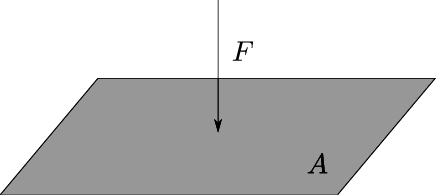
\includegraphics[width=0.5\textwidth]{figs/pression.pdf}
\caption{Une force $F$ appuyant sur une surface $A$.}
\label{fig_FA}
\end{center}
\end{figure} 
Les unités SI de la pression sont des Pascals, 
notés $\Pa$, ou encore des $\N/m^2=\kg/(\m\cdot\s^2)$ (les unités d'une force divisée par une surface).

Un objet au repos dans un fluide subira une pression qui sera la même dans toutes les directions.
Elle est donnée par le poids de la colonne de fluide se trouvant au  dessus de l'objet divisée la surface de l'objet.
Une utilisation très courante de la pression est en météorologie où 
on parle de pression atmosphérique. Elle mesure le poids d'une colonne d'air 
sur le sol par unité de surface. L'unité utilisée pour la pression en météorologie est le $\bar$.
La pression atmosphérique au niveau de la mer est en moyenne d'environ $1\ \bar=10^5\ \N/\m^2$.




\section{Les thermomètres}

La température est une mesure de combien un objet est chaud ou froid. La sensation de chaud ou de froid pour un être humain
est complètement subjective, car dépend de notre système nerveux. On constate donc que pour définir la température il faut définir une 
échelle de référence (tout comme il faut le faire pour la mesure de la distance ou du poids ou de tout autre quantité).

La mesure de la température d'un objet se base sur le fait que de nombreuses propriétés
de la matière peuvent changer avec la température. De façon générale quand on chauffe la matière elle a tendance à occuper un volume plus grand (p. ex. une barre en métal s'allonge lorsqu'on la chauffe). De même les propriétés électriques des conducteurs (leur résistance en particulier) changent avec la température. Finalement la ``couleur'' des objets change avec leur température. La lumière blanche émise par les vieilles ampoules à filament
est obtenue en chauffant un fil en tungstène. 

C'est sur ces principes que sont basés la grande majorité des
thermomètres utilisés dans la vie de tous les jours. Par 
exemple, les thermomètres constitués d'un tube en verre gradué 
rempli d'un liquide (jusque dans les années 1980-90 c'était du mercure, dont l'invention date de 1724, puis c'est devenu de l'alcool). Le liquide se dilate quand il se réchauffe (se contracte quand il se refroidi) et 
donc la hauteur du liquide dans le tube nous donne la température sur l'échelle graduée (voir Figure~\ref{fig_thermo_liquide} où la hauteur du liquide indique environ $29^\circ$ Celsius). Ces thermomètres sont très utilisés pour mesurer la température corporelle ou la température ambiante.
\begin{figure}
\begin{center}
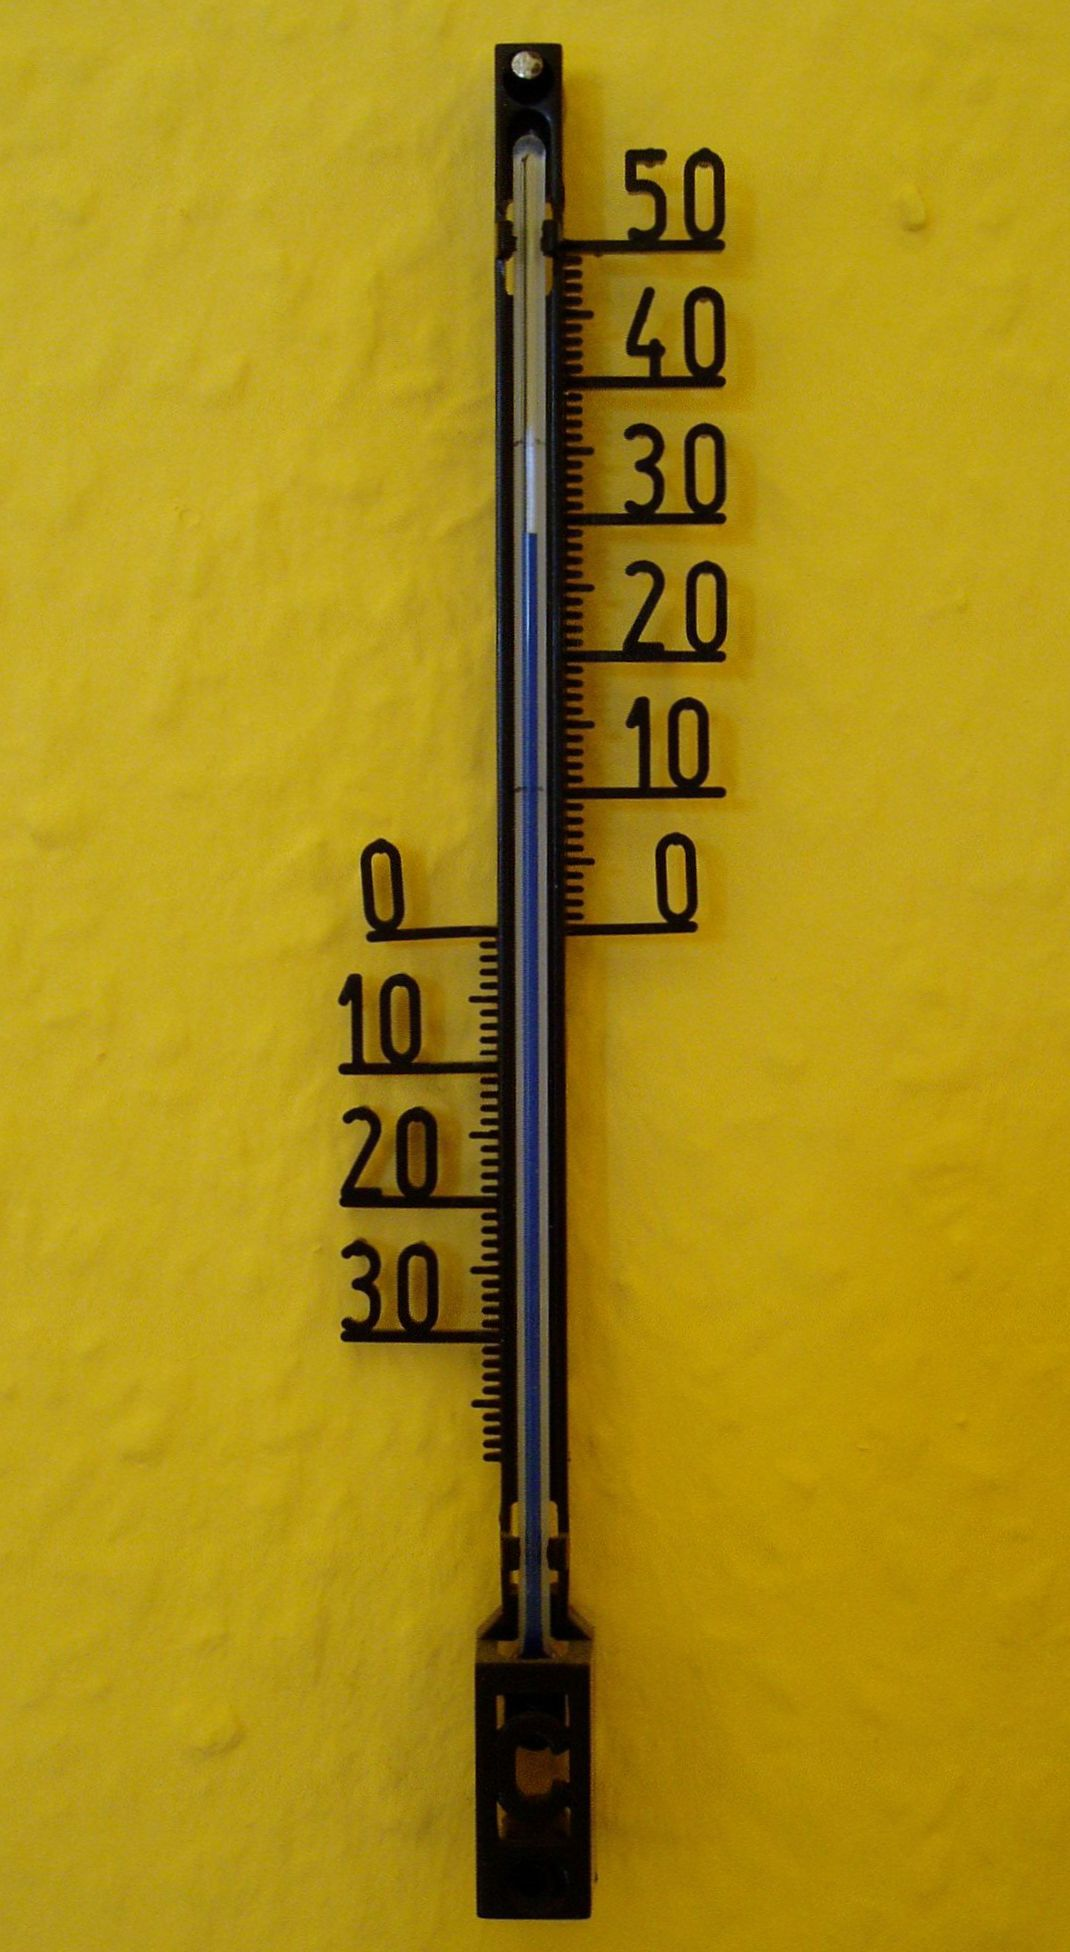
\includegraphics[width=0.5\textwidth]{figs/Thermometer.JPG}
\caption{Thermomètre à liquide avec une échelle allant de $-30^\circ$ à $50^\circ$ degrés Celsius. Source: \url{https://upload.wikimedia.org/wikipedia/commons/3/33/Thermometer.JPG}}
\label{fig_thermo_liquide}
\end{center}
\end{figure} 
Les thermomètres à aiguille (voir Figure~\ref{fig_thermo_aiguille}) sont basés sur la dilatation des solides. 
En général la dilatation d'un solide quand on le chauffe est très faible pour être facilement
visible. Il existe néanmoins des techniques pour ``amplifier'' la dilatation. La première est d'avoir un fil de fer enroulé en spirale 
(la longueur du fil sera donc très longue pour un espace restreint) et l'extrémité centrale de la spirale
fixée sur un axe. De cette façon en fixant une aiguille sur l'autre extrémité du fil la dilatation se transforme en rotation de 
l'aiguille et permet la lecture d'une température. Une autre technique consiste à utiliser le fait que différents matériaux 
se dilatent plus ou moins quand on les chauffe. En soudant donc deux métaux avec un coefficient de dilatation différent, 
l'objet obtenu va se tordre. Ce genre de thermomètres sont utilisés dans les bouilloires par exemple pour déclencher 
l'interrupteur qui arrête le chauffage de l'eau lorsque l'eau bout.
\begin{figure}
\begin{center}
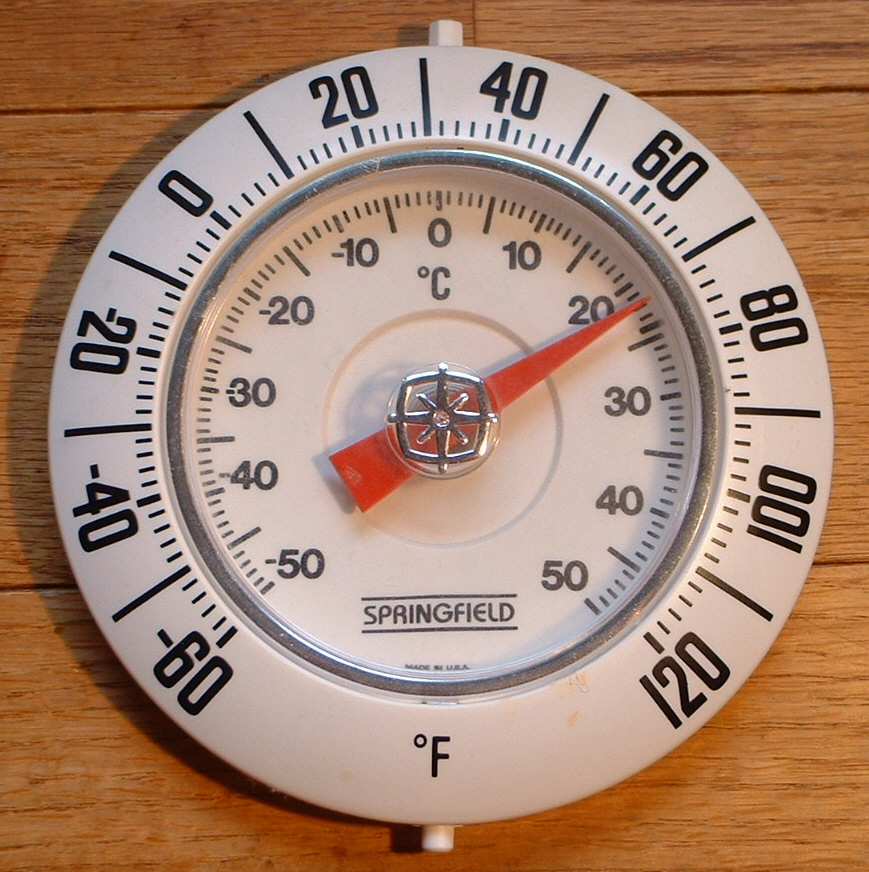
\includegraphics[width=0.5\textwidth]{figs/thermo_c_f.jpg}
\caption{Thermomètre à aiguille avec une échelle allant de $-50^\circ$ à $50^\circ$ degrés Celsius (bague interne) et de $-60^\circ$ à $120^\circ$ 
degrés Fahrenheit. Source: \url{https://upload.wikimedia.org/wikipedia/commons/c/c9/Raumthermometer_Fahrenheit\%2BCelsius.jpg}}
\label{fig_thermo_aiguille}
\end{center}
\end{figure} 
Finalement mentionnons également les thermomètres à infrarouge qui sont basés sur la mesure du rayonnement lumineux (mais pas forcément visible à l’œil nu)
émis par tout corps. La ``couleur'' de ce rayonnement dépend de son énergie. Ces thermomètres fonctionnent donc en mesurant 
l'énergie émise par un corps. Ces thermomètres ont l'avantage de pouvoir mesurer la température à distance (pas besoin d'avoir un contact physique avec la source) contrairement aux deux sortes de thermomètres décrits précédemment. Ils sont utilisés pour mesurer
la température émise par les bâtiments (et donc la déperdition d'énergie associée) ou de chats (voir Figure~\ref{fig_thermographie}).
\begin{figure}
\begin{center}
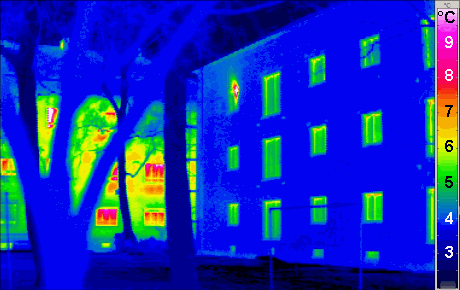
\includegraphics[width=0.5\textwidth]{figs/mais_infra.png}\quad 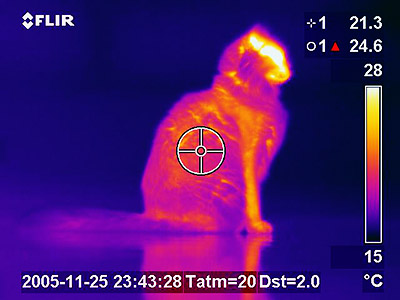
\includegraphics[width=0.42\textwidth]{figs/Termografia_cat.jpg}
\caption{Mesure de température de bâtiments bien isolés ou non (gauche) et de chat (droite). Sources: \url{https://commons.wikimedia.org/wiki/File\%3APassivhaus_thermogram_gedaemmt_ungedaemmt.png}, \url{https://upload.wikimedia.org/wikipedia/commons/8/8e/Termografia_kot.jpg}}
\label{fig_thermographie}
\end{center}
\end{figure}  

\subsection{Les échelles de température}

Nous avons vu ci-dessus comment mesurer une température. Hors nous n'avons pas encore vu comment définir l'échelle 
avec laquelle comparer ces températures et donc comment \textit{calibrer} les thermomètres. 

Il existe trois échelles de température. L'échelle Celsius (utilisée dans la plupart des pays dans la vie de tous les jours), 
l'échelle Fahrenheit (utilisée aux USA principalement) et l'échelle Kelvin qui est utilisée pour les travaux scientifiques
principalement. Historiquement les échelles Celsius et Fahrenheit ont été définies en définissant
de façon arbitraire deux températures de référence. Ces températures ont comme condition qu'elles doivent être facilement reproductibles
et ne pas changer avec les conditions atmosphériques. 

Pour l'échelle Celsius, le $0^\circ$ est défini comme la température de fusion de la glace, et le $100^\circ$ comme la température
d'ébullition de l'eau. Il y a naturellement 100 graduations intermédiaires. Pour l'échelle Fahrenheit, le zéro a été défini comme la température
atteinte par une mixture frigorifique (un mélange de glace d'eau et de chlorure d'ammonium dont la température se stabilise toute seule)
et le $96^\circ$ comme la température du corps humain. Plus tard le standard a été changé. Le $32^\circ$ est devenu la température de
fusion de la glace et le $212^\circ$ la température d'ébullition de l'eau. On peut donc assez facilement convertir les degrés Fahrenheit en 
degrés Celsius.
\begin{exercice}{Conversion de Celsius en Fahrenheit}

\begin{enumerate}
\item Déterminer la formule pour convertir une température en degrés Celsius en degrés Fahrenheit et vice-versa.
\item Calculer la température où la température en degrés Celsius est la même qu'en degrés Fahrenheit ($T_C=T_F$).
\end{enumerate}
\end{exercice}

Une fois qu'une échelle a été définie chaque thermomètre nécessite une étape de calibration. 
Pour les thermomètres de tous les jours, ces calibrations sont 
en général effectuées en plongeant le thermomètre dans un mélange d'eau et de glace suffisamment longtemps pour que 
la température du thermomètre se stabilise. On notera alors que l'état du thermomètre est à la température zéro. Puis 
ont fera de même avec un bain contenant un mélange de vapeur et d'eau liquide. L'état du thermomètre sera la température 100. 
Finalement il suffit de faire 99 graduations entre ces deux températures et le thermomètre est calibré (on peut rajouter des graduation de même taille au delà de l'intervalle 0-100). Néanmoins, chaque thermomètre a ses limitations en termes des températures qu'il peut effectivement mesurer
et la graduation ne peut donc pas se faire ``à l'infini''. Par exemple,
un thermomètre à liquide ne peut pas mesurer une température au-delà de sa température d'ébullition ou en deçà de 
sa température de fusion. De même un thermomètre en spirale ne peux pas mesurer la température au delà de 
la température de fusion du métal dont il est composé.

\subsection{L'équilibre thermique}

La mesure de la température se base sur le fait que lorsque nous mettons deux objets de températures différentes en contact
il vont s'échanger de l'énergie thermique. Un des objets va se réchauffer et l'autre se refroidir jusqu'à ce qu'ils aient la même température.
Lorsqu'ils ont atteint la même température on dit qu'ils sont en \textit{équilibre thermique} et donc il n'y a plus d'échange d'énergie entre eux.

L'équilibre thermique est à la base de la loi zéro de la thermodynamique qui dit que si deux systèmes sont en équilibre thermique avec un troisième système alors ils le sont également entre eux.

La température détermine donc si un système est en équilibre thermique avec un autre (deux systèmes qui ont la même température sont en équilibre thermique).

\section{La dilatation thermique}

Comme nous l'avons dit dans la section précédente, la plupart des substances se dilatent quand elles sont chauffées
et se contractent quand elles sont refroidies. 
Néanmoins, toutes ne le font pas de la même façon. Dans cette section, nous allons étudier la façon dont 
nous pouvons décrire l'augmentation (ou diminution) du volume dû à l'augmentation (ou diminution) de la température.

\subsection{La dilatation linéique}

Considérons un cylindre de longueur $L_0$ qui est à température $T_0$. 
Nous souhaitons connaître la longueur $L$ du cylindre lorsque la température du cylindre est changée 
et donnée par $T$ (voir la Figure~\ref{fig_rods})
\begin{figure}
\begin{center}
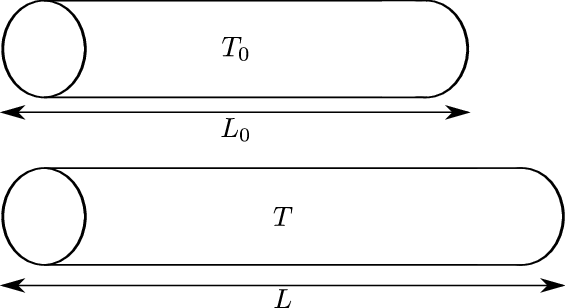
\includegraphics[width=0.3\textwidth]{figs/rods.pdf}
\caption{La longueur du cylindre de longueur $L_0$ à température $T_0$ devient de longueur $L$ lorsqu'il est 
amené à température $T$.}
\label{fig_rods}
\end{center}
\end{figure}
Expérimentalement, on a déterminé que la variation de longueur est reliée linéairement à la variation de température
\begin{equation} 
\Delta L=\alpha L_0\Delta T,\label{eq_dl_dt}
\end{equation}
où $\Delta L=L-L_0$, $\Delta T=T-T_0$, et $\alpha$ est le coefficient de dilatation linéique (qui est constant ici)
dont les unités sont des $^\circ \C^{-1}$. On voit donc que
plus le cylindre est long plus sa longueur variera.
On peut réécrire cette équation pour obtenir 
la longueur finale du cylindre
\begin{equation}
L=L_0+L_0\alpha\Delta T=L_0\left(1+\alpha \Delta T\right).
\end{equation}
On constate que pour $\alpha>0$ le cylindre voit sa taille augmenter lorsqu'on le chauffe.

Cette ``loi'' est une bonne approximation pour autant que
la variation de longueur soit petite (et donc que la 
variation de température soit petite). En particulier
le coefficient de dilatation dépend en général de la
température (voir Figure~\ref{fig_alpha_aciers} pour le coefficient de dilatation linéique de différents types d'acier).
\begin{figure}
\begin{center}
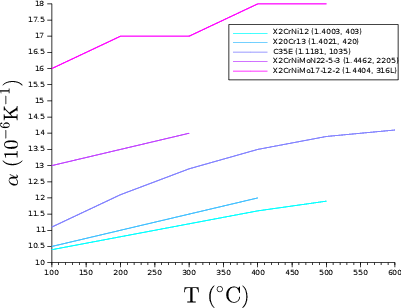
\includegraphics[width=0.5\textwidth]{figs/alpha_aciers.pdf}
\caption{Coefficients de dilatation linéique de différents type d'acier en fonction de la température. Source: \url{https://upload.wikimedia.org/wikipedia/commons/b/b2/Coefficient_dilatation_lineique_aciers.svg}}
\label{fig_alpha_aciers}
\end{center}
\end{figure}

\begin{exercice}{Allongement du pont du Mont-Blanc}

Sachant que les température les plus extrêmes enregistrées à Genève ont été de $-25^\circ\C$ et de $40^\circ\C$, de quelle longueur doivent être les joints de dilatation du Mont-Blanc, sachant qu'il est construit en béton ($\alpha_{\mbox{béton}}=10^{-5}\C^{-1}$) et qu'à une température de $20^\circ\C$ il mesure $252\m$ de long?
\end{exercice}

Il est important de noter que pour un liquide ou un gaz 
la notion de dilatation linéique ne fait pas de sens car lorsqu'elle se trouve dans un de ces états la matière n'a pas de forme précise, contrairement à l'état solide.

\subsection{La dilatation volumique}

La variation du volume d'un matériaux a un comportement très similaire à la dilatation linéique. En fait lorsqu'on varie 
la température d'un objet dont le volume est de $V_0$ à une température $T_0$, on obtient sa variation de volume par la formule suivante
\begin{equation}
\Delta V=\beta V_0\Delta T,
\end{equation}
où $\Delta V=V-V_0$ et $\beta$ est le coefficient de dilatation volumique (encore une fois supposé constant). Lorsque le matériaux est dit isotrope (c'est-à-dire qu'il a les même propriétés dans toutes les directions) les coefficient de dilatation volumiques et linaires sont approximativement reliés par
\begin{equation}% TODO FAIRE LE CALCUL
\beta=3\alpha.
\end{equation}
Cette relation n'est pas vérifiée si le matériel n'est pas isotrope.

De façon similaire à ce que nous avons fait pour la dilatation linéique, nous pouvons calculer directement la valeur du volume final après avoir  chauffé un objet de volume $V_0$ d'une quantité $\Delta T$
\begin{equation}
V=V_0(1+\beta\Delta T).\label{eq_V_T}
\end{equation}
On constate que pour $\beta>0$ le volume va augmenter lorsqu'on chauffe (pour presque tous les matériaux courant $\beta>0$ sauf pour l'eau qui pour certaines températures voit son coefficient de dilatation devenir négatif, voir Figure\ref{fig_alpha_eau}) alors que pour $\beta<0$ le volume va diminuer lorsqu'on chauffe.
\begin{figure}
\begin{center}
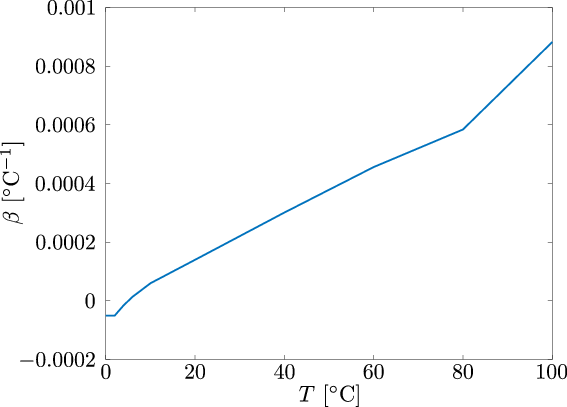
\includegraphics[width=0.5\textwidth]{figs/alpha_eau.pdf}
\caption{Coefficients de dilatation volumique de l'eau en fonction de la température.}
\label{fig_alpha_eau}
\end{center}
\end{figure}

Cette modification du volume en fonction de la température explique également la modification de la masse volumique (ou densité) lorsqu'un objet voit sa température changer. En effet, la densité, $\rho$ est définie par
\begin{equation}
\rho=\frac{m}{V},
\end{equation}
où $m$ est la masse de l'objet. La masse ne changeant pas avec la température (contrairement au volume), en substituant l'équation~\eqref{eq_V_T} dans l'équation ci-dessus, on obtient
\begin{equation}
\rho=\frac{m}{V_0(1+\beta\Delta T)},
\end{equation}
qui est l'équation reliant la densité à la variation de température d'un objet dont le volume est de $V_0$ à température $T_0$.
On constate donc que si $\beta> 0$ la densité diminue avec la température (ce qui explique que l'air chaud a tendance à monter).
Pour la plupart des matériaux $\beta$ est une grandeur qui dépend de la température, mais qui est toujours positive.
Une exception à cette ``règle'' est l'eau. En effet, l'eau a la propriété étonnante de voir sont volume augmenter quand on 
diminue la température ($\beta<0$ entre $0$ et $4$ degrés Celsius). Par ailleurs, autre propriété remarquable, lorsque l'eau se transforme en glace son volume 
augmente également (cela explique l'explosion des bouteilles remplies dans le congélateur, ou de la tuyauterie dans certaines 
vieilles constructions pendant l'hiver).

Cette propriété particulière de l'eau est primordiale
pour la survie des espèces aquatiques pendant l'hiver. 
Prenons l'exemple d'un lac dont la température est supérieure à $4^\circ\C$. Lorsque la température de l'air diminue  en hiver,
la surface de l'eau va se mettre en équilibre thermique avec l'air et voir sa température diminuer. Sa densité
va donc également augmenter jusqu'à ce que sa température atteigne $4^\circ\C$. A cette température la densité de l'eau est maximale. L'eau de la surface va donc avoir tendance à couler
et créer un courant entre la surface et le fond du lac. Ce courant va refroidir le fond du lac et entraîner l'eau plus chaude du lac vers la surface qui va se refroidir à son tour.

Puis, lorsque la température du lac a atteint les $4$ degrés, 
la tempértaure de la surface peut commencer à passer sous les $4^\circ\C$. En dessous de $4^\circ\C$ la densité de l'eau commence à augmenter à nouveau. L'eau refroidie en surface aura donc une densité plus faible que l'eau qui se trouve plus en profondeur. Elle restera donc à la surface du lac. 
Le courant créé précédemment ne sera plus présent. L'eau au fond du lac restera donc plus ``chaude'' beaucoup plus longtemps.
Finalement, quand la surface de l'eau gèlera, la glace qui a une densité également plus faible que l'eau, restera uniquement en surface.
Le lac ne gèlera donc pas entièrement car le fond du lac est d'une certaine façon ``isolé'' de la surface (qui est également la source 
du refroidissement du lac). Évidemment si le froid est trop intense et dure suffisamment longtemps le lac finira par geler quand même
mais il faudra des conditions particulièrement extrêmes.

Si en revanche l'eau n'avait pas ces propriétés exceptionnelles, l'eau froide continuerait à couler depuis la surface jusqu'au fond du lac
accélérant fortement son refroidissement. Pire, quand la surface du lac atteindra des températures négatives, la glace coulera
pour se poser au fond du lac et entraînera la congélation du lac en entier et donc la vie telle que nous la connaissons ne pourrait exister.

\subsection{Contraintes thermiques}

Dans les bâtiments où les routes, la dalle ou les poutres sont en général fixes\footnote{Leur constante de dilatation sera différente du matériaux sur lequel elles sont fixées.} ce qui limite leur possibilité de se dilater/contracter librement lors de changements de température ce qui entraînera l'apparition de contraintes dites thermiques.

Une contrainte est analogue à une pression. Elle correspond à la
force par unité de surface appliquée sur un objet.
SI nous considérons un objet qui va s'allonger (ou se contracter) principalement dans une direction, une contrainte $\sigma$ appliquée sur un objet de longueur $L_0$ a pour effet de l'allonger d'une longueur $\Delta L$. De plus, 
empiriquement on a déterminé que $\sigma$ est proportionnel 
au rapport $\Delta L/L_0$ et la constante reliant les deux quantité s'appelle le module de Young, $E$, (ou module d'élasticité)
\begin{equation}
\sigma=E\frac{\Delta L}{L_0}.
\end{equation}
En utilisant l'équation~\eqref{eq_dl_dt} qui relie $\Delta L$ à $\Delta T$, on obtient
\begin{equation}
\sigma=\alpha E \Delta T.
\end{equation}
On constate donc que la contrainte thermique sur les matériaux est proportionnelle à la variation de température, et dépendante 
de deux constantes que sont le module de Young et le coefficient de dilatation. Comme pour toutes les lois que nous avons vues dans ce chapitre, celle-ci n'est valable que pour les petites variations de température.
\begin{exemple}{Rupture du béton par grande chaleur}

Supposons qu'une autoroute est constituée de blocs de béton
de $10\m$ de long posés côte à côte sans espace entre eux. S'ils ont été posés un jour où la température extérieure est de $10^\circ\C$. Sachant que le module de Young du béton est de $E_{\mbox{béton}}=2\cdot10^{10}\N/\m^2$, 
son coefficient de dilatation linéique est de $\alpha_{\mbox{béton}}=10^{-5}\C^{-1}$, et sa contrainte de rupture en compression est de $\sigma_{\mbox{max}}=2\cdot 10^7 \N/m^2$, est-ce que le béton 
va se rompre par un jour de grande chaleur ($40^\circ\C$)?
\end{exemple}

\section{Lois des gaz et zéro absolu}

Les relations que nous avons vues à la section précédente
ne sont pas valables pour des gaz. En fait, elles ne sont valables que pour les cas où la pression est constante (c'est pour cela que cette grandeur n'apparaît dans aucune des 
équations). Dans le cas des liquides ou des solides la
pression varie en général assez faiblement et l'approximation 
de la pression constante est assez juste. En revanche pour les
gaz la pression peut varier de façon très abrupte\footnote{étant donné qu'ils remplissent totalement le récipient qui les contient il est assez simple de changer dramatiquement la pression d'un gaz}. 

Il nous faut donc généraliser les ``lois'' que nous avons vu précédemment en incluant la pression. Nous allons dériver dans cette section une \textit{équation d'état} reliant la masse, le volume, la pression et la température d'un gaz.  



\subsection{Hypothèses}

Nous allons supposer que le système que nous allons considérer
est en quasi-équilibre: chaque fois que l'état du système est 
modifié (i.e. on fait varier une des quatre variables\footnote{
la masse, la pression, le volume ou la température}) on va 
attendre que le système se remette dans état d'équilibre (il est 
dans un état où plus rien ne varie dans le temps). De plus, les 
résultats de cette section ne sont valables uniquement que
lorsque le gaz n'est pas trop dense ou proche de la liquéfaction.

\subsection{Loi de Boyle-Mariotte}

Robret Boyle et Edme Mariotte ont déterminé expérimentalement au $17^\textrm{\`eme}$
siècle que \textit{lorsqu'on maintient la température d'un gaz constante, on constate que son volume, $V$, varie de façon inversement proportionnelle à sa pression, $P$}
\begin{equation}
V\sim\frac{1}{P},\quad \mbox{pour }T\mbox{ constant.}
\end{equation}
Une autre façon d'écrire la loi de Boyle-Mariotte est 
\begin{equation}
PV= \mbox{cte},\quad \mbox{pour }T\mbox{ constant.}\label{eq_loi_boyle}
\end{equation}
Cela signifie que si nous doublons le volume d'un gaz, sa pression sera divisée par deux. La loi de Boyle-Mariotte 
peut se représenter graphiquement comme sur la figure~\ref{fig_boyle}
où chacune des courbes est la relation entre la pression et le volume pour une température donnée.
\begin{figure}
\begin{center}
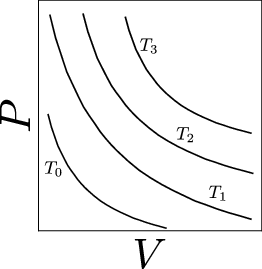
\includegraphics[width=0.5\textwidth]{figs/boyle.pdf}
\caption{Relation entre la pressions $P$ et le volume $V$ pour quatre températures différentes ($T_0$, $T_1$, $T_2$, et $T_3$).}
\label{fig_boyle}
\end{center}
\end{figure}
Autrement dit si un gaz est à température constante $T$ est dans un état d'équilibre avec un volume $V_1$ et
une pression $P_1$ et qu'il y a un autre état d'équilibre avec volume $V_2$ et pression $P_2$ toujours à température $T$ alors l'équation suivante est vérifiée
\begin{equation}
P_1V_1=P_2V_2.
\end{equation}

\begin{exemple}{Plongée sous-marine}

Lors d'une plongée sous-marine on respire l'air à la pression 
de la profondeur à laquelle on se trouve\footnote{Enfin cela est vrai 
si on ne fait pas de la plongée en apnée, où il faut éviter de respirer...}. La pression augmente 
d'environ un bar (environ $10^5\kg\cdot\m^{-1}\s^{-1}$) par dix mètres de profondeur et donc lors de la remontée la pression 
va se réduire fortement. Si on a la mauvaise idée de bloquer sa respiration pendant la remontée, le volume d'air dans les poumons va augmenter fortement car 
\begin{equation*}
V_2=\frac{P_1}{P_2}V_1,
\end{equation*}
où $P_1>P_2$ et donc $V_2>V_1$ (voir la figure \ref{fig_plongee}).
Cette augmentation de volume peut avoir des effets catastrophiques
comme la rupture des tissus des poumons. Moralité, n'oubliez pas d'expirer en remontant à la surface lorsque vous faites de la plongée.

\begin{figure}[htp]
\begin{center}
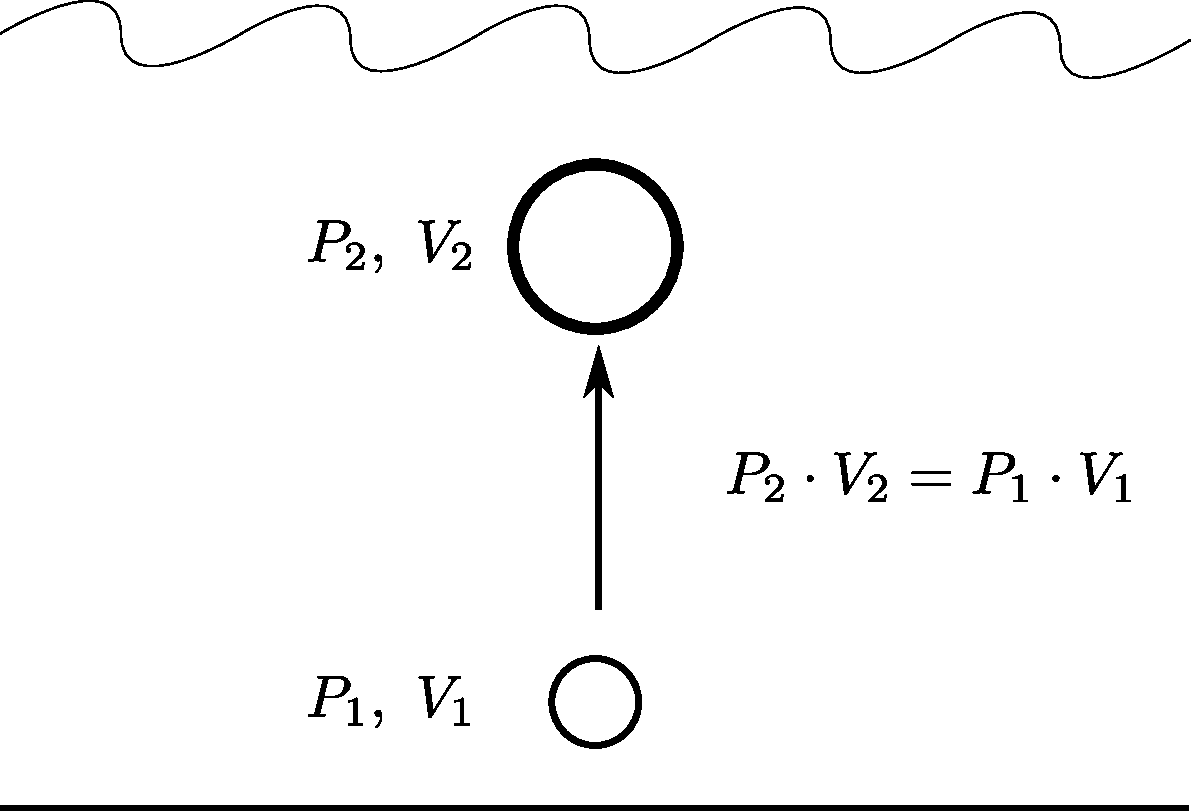
\includegraphics[width=0.5\textwidth]{figs/plongee.pdf}
\caption{Le volume d'un poumon augmente lorsque le plongeur remonte sans expirer passant de $V_2$ à $V_1$.}
\label{fig_plongee}
\end{center}
\end{figure}
\end{exemple}


\subsection{Loi de Charles}

Jacques Charles découvrit au $17^\textrm{\`eme}$ siècle 
qu'à \textit{pression constante le volume d'un gaz est proportionnel à sa température} 
\begin{equation}
V\sim T,\quad \mbox{pour }P\mbox{ constant.}
\end{equation}
ou encore 
\begin{equation}
\frac{V}{T}=\mbox{cte},\quad \mbox{pour }P\mbox{ constant.}\label{eq_loi_charles}
\end{equation}
Autrement dit si un gaz est à pression constante $P$ est dans un état d'équilibre avec un volume $V_1$ et
une température $T_1$ et qu'il y a un autre état d'équilibre avec volume $V_2$ et température $T_2$ toujours à pression $P$ alors l'équation suivante est vérifiée
\begin{equation}
\frac{V_1}{T_1}=\frac{V_2}{T_2}.
\end{equation}
Un exemple pour différents gaz peut être trouvé sur la figure~\ref{fig_charles}.
\begin{figure}
\begin{center}
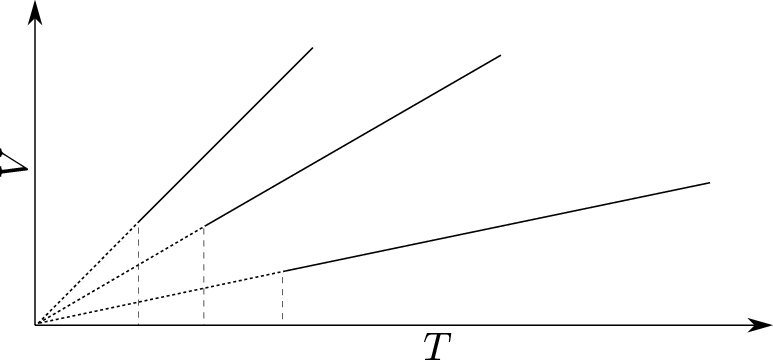
\includegraphics[width=0.5\textwidth]{figs/charles.pdf}
\caption{Relation entre le volume $V$ et la température $T$ à pression constante pour trois gaz. En traitillés, l'extension de la droite au delà du point de liquéfaction du gaz. Toutes les droites se rejoignent au \textit{zéro absolu}.}
\label{fig_charles}
\end{center}
\end{figure}
Chacune des droites représente un gaz différent. Les traits-tillés commencent à l'endroit où le gaz se liquéfie 
(à $0^\circ\C$ pour l'eau, $-183^\circ\C$ pour l'oxygène, ...). 
Dès lors la loi de Charles n'est plus valable. Néanmoins,
il est remarquable de constater que si ces droites sont étendues en-dessous du point de liquéfaction elles se coupent toutes en un point (quel que soit le gaz!): lorsque $V=0$. Ce point théorique se trouve à $-273.15^\circ\C$ et s'appelle le
\textit{zéro absolu}. Le zéro absolu est également le zéro
de l'échelle de Kelvin qui est utilisée dans la plupart des travaux scientifique. L'intervalle du (degré) Kelvin (noté $\K$) est le même que pour les degrés Celsius on a donc
\begin{equation}
T(K)=T(^\circ\C)+273.15.
\end{equation}
A la température de $0\K$ le volume d'un gaz serait nul 
(voire même négatif si on arrivait à descendre plus bas).
Ce genre d'état n'existe à notre connaissance dans la nature et 
défierait toutes les lois telles que nous les connaissons.

Nous avons déjà vu une version de cette loi précédemment (à l'équation~\eqref{eq_V_T}). Une autre façon d'écrire cette loi est
\begin{equation}
V=V_0\left(1+\beta(P)(T-T_0)\right),
\end{equation}
où $\beta(P)$\footnote{dans l'équation~\eqref{eq_V_T}, $\beta$ ne dépendait pas de la pression, car nous considérions un solide, et la presion dans un solide est très difficile à faire changer.} est une fonction de la pression et du gaz considéré 
(en gardant $P$ constant cette valeur ne change pas pour un gaz 
donné), $V_0$ est le volume 
à température de référence $T_0$. Lorsque $P\rightarrow 0$,
$\beta(P)$ devient indépendant du gaz et vaut $1/273.15\ \C^{-1}$.

\subsection{Loi de Gay-Lussac}

Au $19^{\mbox{ème}}$ siècle Joseph Gay-Lussac mis en évidence que \textit{pour un gaz dont le volume est gardé constant, sa pression va varier proportionnellement à sa température}
\begin{equation}
P\sim T,\quad \mbox{pour }V\mbox{ constant.}
\end{equation}
ou encore 
\begin{equation}
\frac{P}{T}=\mbox{cte},\quad \mbox{pour }V\mbox{ constant.}\label{eq_loi_gaylussac}
\end{equation}
Autrement dit si un gaz est à volume constant $V$ est dans un état d'équilibre avec une pression $P_1$ et
une température $T_1$ et qu'il y a un autre état d'équilibre avec pression $P_2$ et température $T_2$ toujours à volume $V$ alors l'équation suivante est vérifiée
\begin{equation}
\frac{P_1}{T_1}=\frac{P_2}{T_2}.
\end{equation}

\subsection{Loi d'Avogadro}

Au $19^{\mbox{ème}}$ siècle Amedeo Avogadro a énoncé que \textit{deux gaz dont la température et la pression sont identiques contiennent exactement le même nombre de molécules}
\begin{equation}
\frac{V_1}{n_1}=\frac{V_2}{n_2},
\end{equation}
où $V_i$ et $n_i$ ($i=1,2$) sont le volume et le nombre de moles des gaz numérotés 1 et 2.
Une autre façon d'exprimer cette loi est de dire qu'à pression et température constante 
le volume $V$ d'un gaz est proportionnel au nombre de moles $n$ qui le constituent
\begin{equation}
V\sim n,\quad \mbox{pour $T,P$ constantes}.
\end{equation}

\subsection{La loi des gaz parfait}

En utilisant les lois de Boyle, Charles et de Gay-Lussac, on peut dériver une loi encore plus générale.
Commençons par réécrire les trois lois (voir les équations \eqref{eq_loi_boyle}, \eqref{eq_loi_charles}, et \eqref{eq_loi_gaylussac})
\begin{align}
PV&=k_T(T),\label{eq_boyle}\\
\frac{V}{T}&=k_P(P),\label{eq_charles}\\
\frac{P}{T}&=k_V(V)\label{eq_gaylussac},
\end{align}
où $k_T,k_P,k_V$ sont trois ``constantes'' où respectivement on suppose qu'on garde la température, 
la pression et le volume constants (néanmoins ces constantes ont une valeur différentes pour des valeurs
différentes de température, pression et volume respectivement). En divisant l'équation~\eqref{eq_boyle}
par $T$ on obtient 
\begin{equation}
\frac{PV}{T}=\frac{k_T(T)}{T}.
\end{equation}
Puis en multipliant l'équation~\eqref{eq_charles} par $P$ on obtient
\begin{equation}
\frac{PV}{T}=k_P(P)P.
\end{equation}
Finalement en multipliant l'équation~\eqref{eq_gaylussac} par $V$ on obtient
\begin{equation}
\frac{PV}{T}=k_V(V)V.
\end{equation}
Comme les membres de gauche de ces trois équations sont identiques, on voit que
\begin{equation}
k_V(V)V=k_P(P)P=\frac{k_T(T)}{T}.
\end{equation}
Cette relation doit être vraie pour $T$, $P$ et $V$ quelconques. 
Ces trois variables étant indépendantes, nous pouvons choisir 
un $V_0$ pour le membre de gauche de l'égalité ci-dessus. On aura donc
\begin{equation}
k_V(V_0)V_0=k_0,
\end{equation}
où $k_0$ est une constante. On voit donc que 
\begin{align}
k_P(P)P=k_0,\\
\frac{k_T(T)}{T}=k_0.
\end{align}
De façon similaire on peut déduire que $k_V(V)V$ est constant.
Finalement, il vient que
\begin{equation}
\frac{PV}{T}=\mbox{cte}.
\end{equation}
Il faut réaliser que par constante, on sous-entend ``qui ne dépend pas de la pression, de la température ou du volume''.
En revanche, il est certain que le membre de droite de cette équation est dépendant de la quantité de gaz
que nous considérons. Souvenons-nous donc de la loi d'Avogadro. On a qu'à pression et température constante,
le volume de gaz est proportionnel au nombre de moles, $n$, dont il est composé. L'équation ci-dessus devient donc
\begin{equation}
\frac{PV}{T}\sim n.
\end{equation}
Expérimentalement, on a déterminé que la relation est en fait donnée par
\begin{equation}
PV=nRT,
\end{equation}
où $R=8.314\ \J/(\mol\cdot\K)$ est la \textit{constante des gaz parfaits} qui est universelle et donc indépendante du type de gaz.

Il est important de noter que la loi du gaz parfait fait intervenir la température en degrés Kelvin (et non en degrés Celsius ou en Fahrenheit). En effet, si $T$ pouvait devenir négatif, on pourrait se retrouver avec un volume négatif ce qui
n'aurait aucun sens physique.

\subsection{Limitations}

La loi des gaz parfaits est une approximation des gaz réels qui n'est valable que 
sous certaines conditions
\begin{enumerate}
\item Le gaz doit être dans un état d'équilibre.
\item Le gaz ne doit pas être trop proche de son point de liquéfaction.
\item La pression du gaz doit être ``faible'' ($P\leq 1\ \bar$).
\item Le gaz n'est pas en train de subir une réaction chimique.
\end{enumerate}
Néanmoins, sous ces conditions il représente très bien ce qui se passe dans plus ou moins tous les gaz connus.

\begin{exemple}{Volume d'une mole de gaz}

Estimer le volume d'une mole d'un gaz à $T=0^\circ\C$, $P=10^5\ N/\m^2$. Et à $T=20^\circ\C$?
\end{exemple}
\begin{solution}
En utilisant la loi des gaz parfaits on a
\begin{align*}
&10^5\cdot V=1\cdot 8.314\cdot 273,\\
&V=8.314\cdot 273\cdot 10^{-5},\\
&V=0.0227\ \m^3.
\end{align*}
Et à $20^\circ\C$
\begin{align*}
&10^5\cdot V=1\cdot 8.314\cdot 293,\\
&V=8.314\cdot 293\cdot 10^{-5},\\
&V=0.0244\ \m^3.
\end{align*}
\end{solution}

\begin{exercice}{Gaz parfaits}
\begin{enumerate}
\item Estimer la masse d'air dans une salle dont les dimensions sont $15\m\times 10\m\times 3\m$ à une température $T=20^\circ\C$
à une pression de $P=1.013\cdot 10^5\ N/\m^2$. A combien de moles cela correspond-il? Quelle est la densité de l'air dans la salle?


\item Un ballon d'hélium (qu'on suppose avoir la forme d'une sphère parfaite) a un rayon de $18\cm$. A $20^\circ\C$
la pression interne du ballon est de $1.064\cdot 10^5\N/m^2=1.05\atm$. Calculer le nombre de moles, la masse et la densité de l'hélium dans le ballon.

\item Le ballon flotte-t-il? Quelle devrait être la pression du ballon pour que l'hélium ait la même densité que l'air?
\end{enumerate}
\end{exercice}


\chapter{Chaleur et matière}

Lorsqu'on chauffe une casserole d'eau froide sur la plaque du cuisinière (qui n'est pas à induction), la température de l'eau augmente.. 
On dit qu'il y a un flux de ``chaleur'' entre la plaque et l'eau froide. De façon générale lorsque deux objets ont une température différente et qu'on les mets en contact, 
nous considérons que la chaleur va se transférer 
de l'objet chaud à l'objet froid afin d'égaliser la température entre les deux. Après un certain temps les deux objets auront la même
température. On dira qu'ils sont en \textit{équilibre thermique}.
A ce moment là il n'y aura plus d'échange de chaleur entre les deux objets (le flux est interrompu). 

Dans ce chapitre nous allons définir le concept de chaleur (qui
est différent de celui de température!). Puis verront les effets 
de la chaleur sur la matière (notamment sur les transitions de phase) et les processus qui permettent de la transférer: 
la conduction, la convection et la radiation.


\section{La chaleur comme un transfert d'énergie}

Au 18-ème siècle la chaleur était vue comme un ```fluide''
qui constituait tout corps chaud et qui pouvait être ``couler''
vers un corps froid. Ce fluide s'appelait le \textit{calorique}. 
Au 19-ème siècle on se rendit compte que ce modèle était faux, en particulier s'il existait, ce fluide devait être sans masse. De plus, on montra que tant qu'on produisait du \textit{travail}
on pouvait continuer à chauffer des objets et donc potentiellement il existerait une ``infinité'' de calorique
ce qui contredisait la théorie du fluide calorique (cela voudrait dire qu'une quantité potentiellement infinie de calorique existait en chaque objet). 

Depuis, la vision que nous avons de la chaleur est celle qui 
l'identifie à la notion de \textit{travail}. 

\subsection{Brève introduction sur le travail}

\subsection{}



\end{document}
